\documentclass[A4paper, 11pt]{article}
\usepackage[slovene]{babel}
\usepackage[utf8]{inputenc}
\usepackage{array}
\usepackage{amsfonts}
\usepackage{pifont}
\usepackage{theorem}
\usepackage{authblk}
\usepackage{url}

\usepackage{graphicx}
\graphicspath{ {slike/} }

\title{Kodiranje s pomočjo sudoku ključa}
\author{Klementina Pirc}
\affil{Fakulteta za matematiko in fiziko \\ Oddelek za matematiko}
\date{26. april 2018}

\newtheorem{definicija}{Definicija}
\theorembodyfont{\mdseries}
\newtheorem{zgled}{Zgled}

\newcommand{\cmark}{\ding{51}}
\newcommand{\xmark}{\ding{55}}

\begin{document}

\begin{titlepage} 

\maketitle
\thispagestyle{empty}
	
\end{titlepage}


% UVOD

\section{Uvod}

V današnjem svetu, kjer se vsak dan preko različnih komunikacijskih kanalov pretoči nepredstavljiva količina informacij, se pojavi vprašanje varovanja osebnih podatkov. Tema je še posebno aktualna na področju spletnih bančnih storitev in drugih zaupnih dejavnostih. Pomagamo si s šifriranjem podatkov, navadno s pomočjo neke metode ali ključa, ki ga poznata le pošiljatelj in prejemnik. Pri šifriranju s ključem naletimo na težavo, kako ključ za dešifriranje na varen način in v realnem času sporočiti našemu sogovorniku. Če namreč prisluškovalec prestreže naš ključ in za tem še sporočilo, bo brez težav dešifriral podatke.

Kvantno šifriranje oziroma kvantna kriptografija temelji na posebnih fizikalnih lastnostih delcev. Te lastnosti omogočajo varen prenos šifrirnega ključa tudi preko javnega, nezaščitenega komunikacijskega kanala. S pomočjo te metode lahko celo ugotovimo, ali je bila med pošiljateljem in prejemnikom prisotna tretja oseba, in po potrebi pripravimo nov ključ za šifriranje.


%POLARIZACIJA FOTONOV

\section{Polarizacija fotonov}

\subsection{Foton}

Definirajmo najprej nekaj osnovnih pojmov s področja fizike delcev in fizike na splošno.

\begin{definicija}
Osnovni delec je delec, ki nima podstrukture, torej ni sestavljen iz manjših delcev.
\end{definicija}

\begin{definicija}
Svetloba je elektromagnetno valovanje pri različnih valovnih dolžinah oziroma frekvencah.
\end{definicija}

\begin{definicija}
Foton je brezmasni in električno nevtralen osnovni delec, ki potuje s svetlobno hitrostjo in je osnovni gradnik svetlobe.
\end{definicija} 

Torej si lahko širjenje svetlobe oziroma elektromagnetnega valovanja predstavljamo kot gibanje velikega števila fotonov v določeni smeri. Energija fotonov se spreminja obratno sorazmerno glede na valovno dolžino izsevane svetlobe. Tako krajša valovna dolžina pomeni več energije.

\pagebreak

\subsection{Polarizacija svetlobe}

\begin{definicija}
Polarizacija valovanja opisuje smer nihanja količine, ki valuje.
\end{definicija}

\begin{figure}[h]
\centering
\caption{Primer polarizacije}
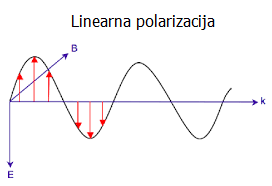
\includegraphics[scale=0.75]{1}
\end{figure}

S polarizacijo opisujemo le transverzalno valovanje, saj pri longitudinalnem smer nihanja količine sovpada s smerjo valovanja. Poznamo tri osnovne tipe polarizacije: linearno, krožno in eliptično.

\begin{definicija}
Val je linearno polariziran, če nihanje poteka le v eni smeri. Krožno in eliptično polarizacijo dobimo, kadar se s širjenjem vala nihanje suče.
\end{definicija}

\begin{figure}[h]
\centering
\caption{Osnovni tipi polarizacije}
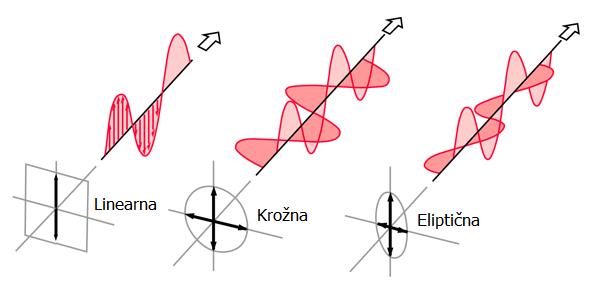
\includegraphics[scale=0.7]{3}
\end{figure}

\pagebreak

Če se smer nihanja neurejeno obrača v vse smeri, govorimo o nedoločeni polarizaciji oziroma nepolariziranem valovanju. Takšno je naprimer svetloba, ki jo oddajajo navadna svetila pa tudi Sonce. \\

Elektromagnetno valovanje oziroma svetloba je transverzalno valovanje. Sestavljeno je iz nihanja električnega in magnetnega polja, ki nihata pravokotno na smer valovanja ter pravokotno en na drugega. Po dogovoru je smer polarizacije enaka smeri nihanja jakosti električnega polja.

\begin{figure}[h]
\centering
\caption{Elektromagnetno valovanje}
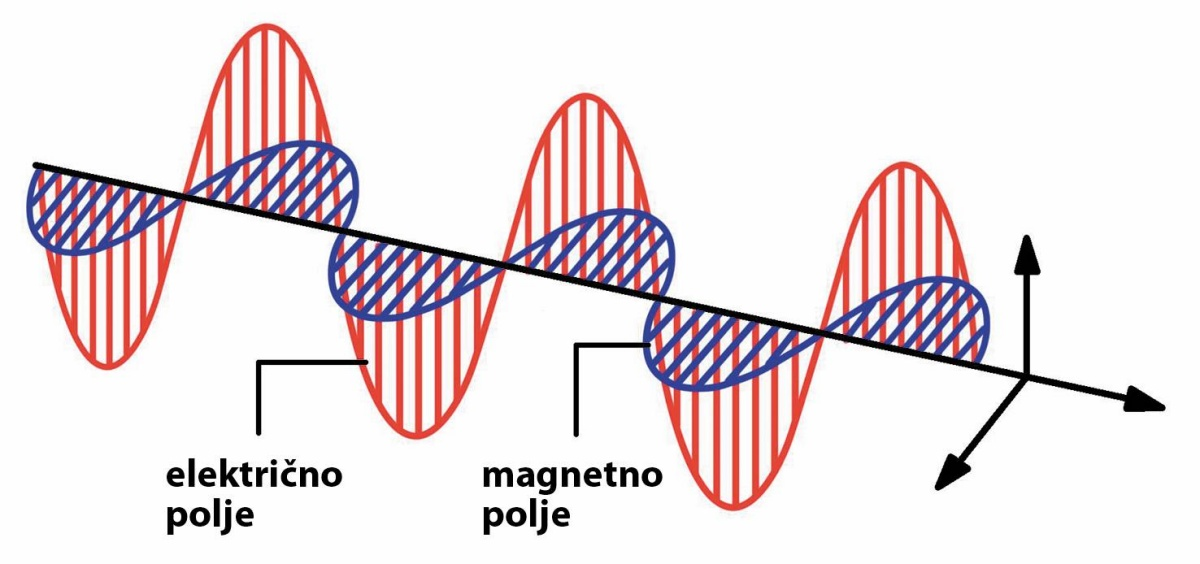
\includegraphics[scale=0.7]{emv}
\end{figure}

V nadaljevanju bomo potrebovali linearno polarizacijo fotonov, zato si poglejmo, kako jo lahko umetno ustvarimo. Naj še enkrat opomnimo, da polarizacija fotonov sovpada s polarizacijo elektromagnetnega valovanja. 

\begin{definicija}
Polarizator je naprava, ki valovanje z nedoločeno ali mešano polarizacijo spremeni v valovanje z določeno polarizacijo.
\end{definicija}

\begin{figure}[h]
\centering
\caption{Delovanje polarizatorja}
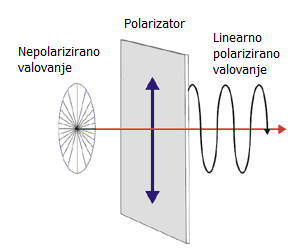
\includegraphics[scale=0.8]{2}
\end{figure}

\pagebreak


%KVANTNA RAZDELITEV KLJUČA

\section{Kvantna razdelitev ključa} \label{kvantna_razdelitev}

\begin{definicija}
Šifriranje podatkov je pretvorba podatkov v obliko, ki je nepooblaščene osebe ne razumejo.
\end{definicija}

Navadno šifriramo podatke z uporabo algoritmov ter drugih matematičnih postopkov. Čeprav je lahko tak postopek zelo učinkovit in ga morebitni vsiljivci težko dešifrirajo, pa je skoraj nemogoče preveriti prisotnost prisluškovalca. Prav to je izjemna lastnost kvantnega šifriranja podatkov. Sogovornika namreč ob koncu pogovora vesta, ali je njuno sporočila prejela še tretja oseba.

Kvantna razdelitev ključa lahko poteka na več različnih načinov, ogledali si bomo postopek, ki ustreza protokolu BB84.

Za lažjo razlago postopka poimenujmo udeležence pri prenašanju sporočila.

\begin{definicija}
Alica je pošiljatelj sporočila.\\
Bob sporočilo prejme.\\
Eva pa ga skuša prestreči, torej je prisluškovalka.
\end{definicija}

Kako poteka kvantno šifriranje?\\
Spoznali smo že fotone, njihovo polarizacijo in izvedeli, kako lahko polarizacijo spreminjamo. Torej lahko z različnimi polarizacijami fotonov predstavimo različne vrednosti.

\begin{zgled}
Naj linearna polarizacija v smeri y osi ($\uparrow$) v binarnem zapisu pomeni $1$, polarizacija v smeri x osi ($\rightarrow$) pa $0$. Na ta način lahko Alica z zaporedjem fotonov, ki jim priredi polarizacijo, pošlje Bobu število v binarnem zapisu. Zaporedje fotonov s polarizacijo $\uparrow$ $\rightarrow$ $\uparrow$ $\uparrow$ $\rightarrow$ tako predstavlja število $10110$.
\end{zgled}

Lahko bi definirali še število $2$ s polarizacijo v smeri premice pri kotu $45^{\circ}$ ($\nearrow$) ter število $3$ pri kotu $135^{\circ}$ ($\nwarrow$). Z različnimi smermi polarizacije lahko predstavimo še druge vrednosti in tako šifriramo sporočilo. Vendar je bolj enostavno, če se omejimo na manjše število polarizacij in uporabimo kvantno šifriranje izključno za pošiljanje ključa, s katerim nato šifriramo nadaljnja sporočila. \\

Bob mora pri prejemu posameznega fotona uporabiti ustrezen polarizator, sicer odčitana vrednost ni pravilna. Če je Alica foton polarizirala z $\uparrow$ ali $\rightarrow$, mora za pravilno interpretacijo Bob uporabiti polarizator oblike $+$, za $\nearrow$ in $\nwarrow$ polarizaciji pa polarizator $\times$. Taki obliki polarizatorja namreč omogočata nemoteno prehajanje fotonov z ustreznimi polarizacijami. Polarizatorjem določene oblike pravimo tudi baza polarizacije. Polarizator $+$ je torej baza polarizacije za polarizaciji $\uparrow$ in $\rightarrow$. Kaj bi se zgodilo, če bi Bob pri prejemu fotona uporabil napačen polarizator?

\begin{zgled}
Recimo, da želi Alica poslati vrednost $1$, torej pošlje foton s polarizacijo $\uparrow$. Če Bob namesto polarizatorja $+$, ki bi pravilno odčital polarizacijo fotona, uporabi polarizator $\times$, bo naključno prejel eno od polarizacij $\nearrow$ in $\nwarrow$. Torej bo namesto vrednosti $1$ prejel število $2$ ali $3$ oziroma ustrezno definirano vrednost pri posamezni polarizaciji.
\end{zgled}

Pojavi se vprašanje, kako naj bi Bob vedel, kateri polarizator mora uporabiti. Alica mu zaradi morebitne prisotnosti Eve seveda ne sme povedati, katero polarizacijo je uporabila na fotonih. Odgovor je preprost: tudi Bob ne ve, kateri polarizator mora uporabiti, zato ga kar naključno izbere. Skoraj zagotovo torej Alica in Bob po koncu pošiljanja fotonov nimata enakega ključa. Komunikacijo lahko nadaljujeta po nevarovanem kanalu, pri čemer Alica Bobu pove, kateri polarizator je ustrezal posameznemu fotonu, ne izda pa točne polarizacije. Bob ji sporoči, pri katerih fotonih je uporabil pravilni polarizator. Fotone, pri katerih nista bila usklajena, enostavno ignorirata in tako dobita končni ključ. \\

\begin{zgled}
Naj bo $\uparrow$ oznaka za $1$ in $\rightarrow$ za $0$ v polarizacijski bazi + ter $\nwarrow$ oznaka za $1$ in $\nearrow$ za $0$ v bazi $\times$.


\begin{center}
\begin{tabular}{ l m{0.3 cm} m{0.3 cm} m{0.3 cm} m{0.3 cm} m{0.3 cm} m{0.3 cm} m{0.3 cm} m{0.3 cm} m{0.3 cm} m{0.3 cm} m{0.3 cm} m{0.3 cm}}
vrednost & 1 & 0 & 1 & 1 & 0 & 0 & 1 & 1 & 0 & 0 & 1 & 1 \\
baza polarizacije & + & + & $\times$ & + & $\times$ & $\times$ & $\times$ & + & $\times$ & + & + & $\times$\\
polarizacija & $\uparrow$ & $\rightarrow$ & $\nwarrow$ & $\uparrow$ & $\nearrow$ & $\nearrow$ & $\nwarrow$  & $\uparrow$ & $\nearrow$ & $\rightarrow$ & $\uparrow$ & $\nwarrow$\\
\\
Bobov polarizator & + & $\times$ & + & + & $\times$ & $\times$ & + & + & $\times$ & + & $\times$ & $\times$\\
odčitana polarizacija & $\uparrow$ & $\nearrow$ & $\rightarrow$ & $\uparrow$ & $\nearrow$  & $\nearrow$ & $\uparrow$ & $\uparrow$ & $\nearrow$ & $\rightarrow$ & $\nearrow$ & $\nwarrow$\\
odčitana vrednost & 1 & 0 & 0 & 1 & 0 & 0 & 1 & 1 & 0 & 0 & 0 & 1\\
\\
končni ključ & 1 & - & - & 1 & 0 & 0 & - & 1 & 0 & 0 & - & 1\\
\end{tabular}
\end{center}

\end{zgled}

Zakaj nam torej tak prenos podatkov omogoča zaznavo prisluškovalca?
Če Eva želi dobiti sporočilo, ki ga Alica pošilja Bobu, mora prestreči poslane fotone. Pri tem mora za odčitavanje polarizacij uporabiti enega od polarizatorjev. Eva ne ve, katero polarizacijo je Alica izbrala za posamezen foton, in lahko le naključno izbere polarizator, s katerim bo prebrala foton in ga nato poslala Bobu. Ima torej $50\%$ možnosti, da se pri izbiri zmoti, s tem pokvari prvotno polarizacijo in zato Bobu posreduje napačno polariziran foton. Bob prejme foton in tako kot Eva naključno izbere polarizator. Sledijo štirje možni scenariji.

\begin{enumerate}

\item Tako Eva kot Bob sta pravilno izbrala polarizatorja, zato se polarizacija ohrani in oba odčitata pravilno vrednost fotona (prvi foton v  zgledu \ref{zgled-eva}).

\item Eva je izbrala napačen polarizator in pokvarila prvotno polarizacijo. Bob je izbral enak polarizator kot Eva, torej je odčital njeno naključno spremenjeno polarizacijo, ki se razlikuje od Alicine. Ker imata Alica in Bob v tem primeru različni bazi polarizacije, bosta ta foton zanemarila (drugi foton v  zgledu \ref{zgled-eva}).

\item Eva je izbrala napačen polarizator. Bob je izbral enak polarizator kot Alica, vendar je od Eve prejel spremenjeno polarizacijo, ki ne ustreza njegovi izbiri polarizatorja. Odčital bo naključno polarizacijo iz baze, ki jo je izbral. V polovici primerov te vrste bo prišlo do razlikovanja v vrednosti, kljub temu da sta Alica in Bob uporabila enaki bazi polarizacije (tretji foton v zgledu \ref{zgled-eva}).

\item Zadnja možnost je enaka prejšnji, le da Bob na koncu po naključju odčita pravilno polarizacijo. Alica in Bob imata torej enako vrednost kljub posredovanju Eve (šesti foton v  zgledu \ref{zgled-eva}).

\end{enumerate}

V tretjem primeru bosta torej Alica in Bob pri pregledovanju polarizatorjev pod vtisom, da se njuni vrednosti ujemata, vendar zaradi Eve temu ni tako. V resnici nimata enakega ključa za šifriranje, zato Bob prejetega sporočila ne bo mogel dešifrirati s svojim ključem. Tako bosta vedela, da je bila med pošiljanjem ključa prisotna Eva.

\pagebreak

\begin{zgled} \label{zgled-eva}
Primer z Evino prisotnostjo.

\begin{center}
\begin{tabular}{ l m{0.3 cm} m{0.3 cm} m{0.3 cm} m{0.3 cm} m{0.3 cm} m{0.3 cm} m{0.3 cm} m{0.3 cm}}
vrednost & 0 & 1 & 1 & 0 & 1 & 0 & 0 & 1\\
baza polarizacije & + & + & $\times$ & + & $\times$ & $\times$ & $\times$ & + \\
polarizacija & $\rightarrow$ & $\uparrow$ & $\nwarrow$ & $\rightarrow$ & $\nwarrow$ & $\nearrow$ & $\nearrow$  & $\uparrow$\\
\\
Evin polarizator & + & $\times$ & + & + & $\times$ & + & $\times$ & +\\
nova polarizacija & $\rightarrow$ & $\nearrow$ & $\uparrow$ & $\rightarrow$ & $\nwarrow$  & $\uparrow$ & $\nearrow$ & $\uparrow$\\
\\
Bobov polarizator & + & $\times$ & $\times$ & $\times$ & + & $\times$ & + & +\\
odčitana polarizacija & $\rightarrow$ & $\nearrow$ & $\nearrow$ & $\nwarrow$ & $\uparrow$  & $\nearrow$ & $\rightarrow$ & $\uparrow$\\
odčitana vrednost & 0 & 0 & 0 & 1 & 1 & 0 & 0 & 1\\
\\
končni ključ & 0 & - & 0 & - & - & 0 & - & 1\\
ujemanje ključev & \cmark & - & \xmark & - & - & \cmark & - & \cmark\\ 
\end{tabular}
\end{center}

\end{zgled}


%SUDOKU

\section{Sudoku}

\begin{definicija}
Sudoku je logična uganka, pri kateri je cilj zapolniti mrežo velikosti $9\times9$ s števili od $1$ do $9$ tako, da se vsako število v vsakem stolpcu, vrstici in $3\times3$ kvadratu znotraj mreže pojavi natanko enkrat.
\end{definicija}

\begin{figure}[h]
\centering
\caption{Primer rešenega sudokuja}
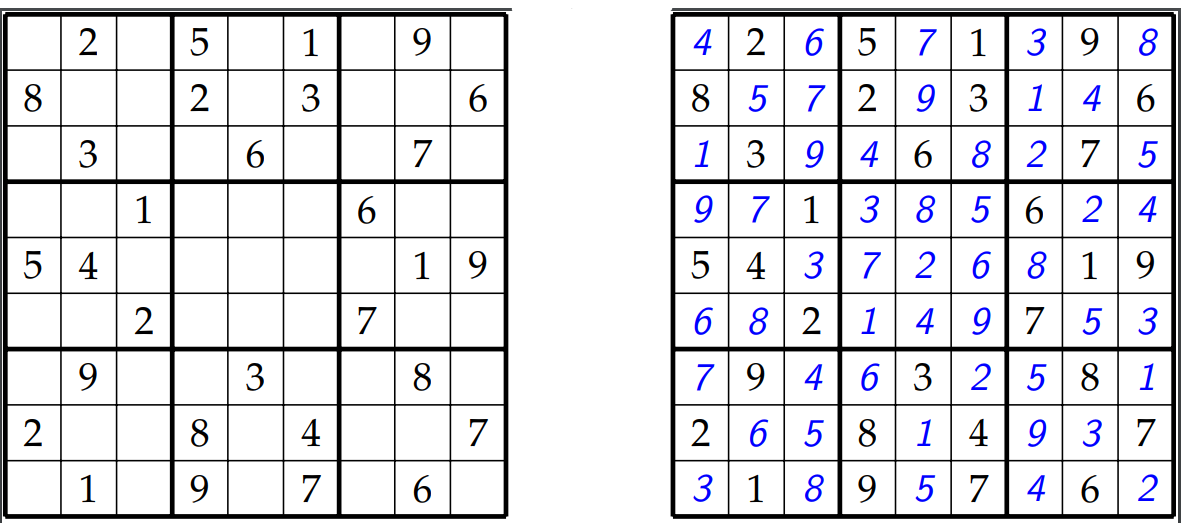
\includegraphics[scale=0.4]{sudoku_resen}
\end{figure}

\pagebreak

Sudokuja se je domislil Američan Howard Garns in ga prvič objavil leta $1979$. Pravijo, da je idejo dobil na podlagi Eulerjevega latinskega kvadrata. To je matrika velikosti $n \times n$, napolnjena z n različnimi znaki, pri čemer se vsak znak v vrstici in stolpcu pojavi natanko enkrat.

Čez $5$ let so uganko objavili tudi na Japonskem in jo poimenovali ''Suuji wa dokushin ni kagiru'', kar v prevodu pomeni ''števke morajo biti edine''. Prvi zlogi besed nam podajo ravno znano ime uganke: SUDOKU.

Število vseh možnih sudoku mrež pri velikosti $9\times9$, je približno $6,6$ trilijonov natančneje $6.670.903.752.021.072.936.960$. Zahtevnost uganke je obratno sorazmerna s številom že vpisanih števil. Lažji sudokuji imajo tako podanih več kot $30$ števil, težji pa nekje med $20$ in $30$. Dolgo je bil odprt problem najmanjšega števila začetnih števil, ki še vedno podajo enolično rešitev. Leta $2012$ so dokazali, da je to število $17$, saj je bilo iskanje enolične rešitve s pomočjo računalnika za sistem s $16$ podanimi števili neuspešno.

Skozi leta so se razvile različne oblike sudokuja in prispevale k težavnosti reševanja. Poznamo naprimer Sudoku X, pri katerem mora poleg standardnih pogojev veljati še, da se števila tudi na diagonalah pojavijo le enkrat. Še bolj ekstremna oblika pa je geometrijski sudoku, pri katerem znotraj mreže nimamo $3\times3$ kvadratov, temveč različne geometrijske like sestavljene iz devetih polj.

\begin{figure}[h]
\centering
\caption{Geometrijski sudoku}
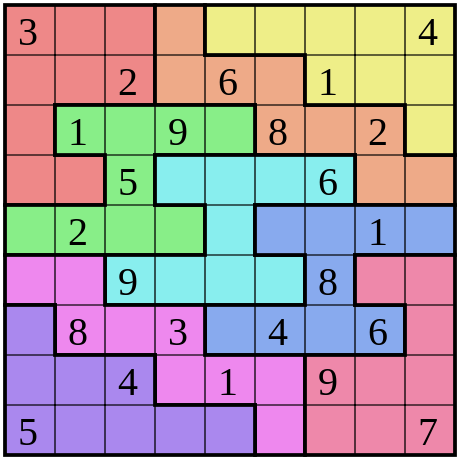
\includegraphics[scale=0.4]{geo_sudoku}
\end{figure}

% SUDOKU KLJUČ

\section{Sudoku ključ} \label{sudoku-kljuc}

Na primeru si oglejmo, kako poteka kvantno razdeljevanje ključa s pomočjo sudoku mreže.

Alica se odloči, da bo ključ za šifriranje poslala Bobu s pomočjo fotonov tako, da bo zaporedje polarizacij predstavljalo rešitev $4\times4$ sudoku mreže. Poslala bo sledeč sudoku:

\begin{center}
\begin{tabular}{| c | c || c | c |}
\hline
0 & 1 & 2 & 3\\
\hline
3 & 2 & 1 & 0\\
\hline
\hline
2 & 0 & 3 & 1\\
\hline
1 & 3 & 0 & 2\\
\hline
\end{tabular}
\end{center}

Pri tem bo uporabila polarizacije:

\begin{center}
\begin{tabular}{l c c c c}
vrednost & 0 & 1 & 2 & 3\\
polarizacija & $\rightarrow$ & $\uparrow$ & $\nwarrow$ & $\nearrow$\\
baza polarizacije & + & + & $\times$ & $\times$\\
\end{tabular}
\end{center}

Če sudoku mrežo pretvorimo v zaporedje fotonov z ustrezno polarizacijo, dobimo:

\begin{center}
\begin{tabular}{l m{0.2 cm} m{0.2 cm} m{0.2 cm} m{0.2 cm} m{0.2 cm} m{0.2 cm} m{0.2 cm} m{0.2 cm} m{0.2 cm} m{0.2 cm} m{0.2 cm} m{0.2 cm} m{0.2 cm} m{0.2 cm} m{0.2 cm} m{0.2 cm}}
vrednost & 0 & 1 & 2 & 3 & 3 & 2 & 1 & 0 & 2 & 0 & 3 & 1 & 1 & 3 & 0 & 2\\
baza & + & + & $\times$ & $\times$ & $\times$ & $\times$ & + & + & $\times$ & + & $\times$ & + & + & $\times$ & + & $\times$\\
polarizacija & $\rightarrow$ & $\uparrow$ & $\nwarrow$ & $\nearrow$ & $\nearrow$ & $\nwarrow$ & $\uparrow$ & $\rightarrow$ & $\nwarrow$ & $\rightarrow$ & $\nearrow$ & $\uparrow$ & $\uparrow$ & $\nearrow$ & $\rightarrow$ & $\nwarrow$
\end{tabular}
\end{center}

Po prej opisanem postopku (poglavje \ref{kvantna_razdelitev}) Alica Bobu pošlje fotone, on pa jih prestreže in na vsakem uporabi naključno izbrano bazo polarizacije, torej $+$ ali $\times$. 

\begin{center}
\begin{tabular}{l m{0.2 cm} m{0.2 cm} m{0.2 cm} m{0.2 cm} m{0.2 cm} m{0.2 cm} m{0.2 cm} m{0.2 cm} m{0.2 cm} m{0.2 cm} m{0.2 cm} m{0.2 cm} m{0.2 cm} m{0.2 cm} m{0.2 cm} m{0.2 cm}}
vrednost & 0 & 1 & 2 & 3 & 3 & 2 & 1 & 0 & 2 & 0 & 3 & 1 & 1 & 3 & 0 & 2\\
baza & + & + & $\times$ & $\times$ & $\times$ & $\times$ & + & + & $\times$ & + & $\times$ & + & + & $\times$ & + & $\times$\\
polarizacija & $\rightarrow$ & $\uparrow$ & $\nwarrow$ & $\nearrow$ & $\nearrow$ & $\nwarrow$ & $\uparrow$ & $\rightarrow$ & $\nwarrow$ & $\rightarrow$ & $\nearrow$ & $\uparrow$ & $\uparrow$ & $\nearrow$ & $\rightarrow$ & $\nwarrow$\\
\\
Bobova baza & + & $\times$ & + & + & $\times$ & $\times$ & + & $\times$ & + & $\times$ & $\times$ & + & $\times$ & $\times$ & $\times$ & $\times$\\
prejeta vrednost & 0 & - & - & - & 3 & 2 & 1 & - & - & - & 3 & 1 & - & 3 & - & 2\\ 
\end{tabular}
\end{center}

Bob lahko vrednosti, pri katerih sta se njegova in Alicina baza polarizacije ujemali, vnese v $4\times4$ mrežo in na ta način dobi nerešen sudoku.

\begin{center}
\begin{tabular}{| c | c || c | c |}
\hline
0 & & & \\
\hline
3 & 2 & 1 & \\
\hline
\hline
& & 3 & 1\\
\hline
& 3 & & 2\\
\hline
\end{tabular}
\end{center}

Sudoku reši po pravilih reševanja in dobi celoten ključ za šifriranje. Minimalno število podanih števil za enolično rešitev sudokuja velikosti $4\times4$ je $4$, kar pomeni, da mora Bob pravilno odčitati polarizacije vsaj štirih fotonov. V nasprotnem primeru je treba postopek ponoviti, seveda z novim ključem.

Če je bila pri prenašanju ključa prisotna tudi Eva, bo pokvarila postavitev števil, ki omogoča pravilno rešitev sudokuja, in tako razkrila svojo prisotnost. Bob namreč ne bo mogel rešiti sudoku mreže na način, ki bi ustrezal pravilom.


% ZAKLJUČEK

\section{Zaključek}

Prednost pošiljanja ključa za šifriranje s pomočjo sudokuja je v tem, da Bobu ni treba povedati, pri katerih fotonih je izbral pravilni polarizator. Slaba lastnost se skriva v tem, da tudi Eva pozna postopek, s katerim dobi celoten ključ. Pravilno mora odčitati le zadostno število polarizacij, torej v našem zgledu $4$ (poglavje \ref{sudoku-kljuc}).

Seveda pa ne smemo pozabiti, da bo Eva s svojim posredovanjem v večini primerov pokvarila pravilno postavitev sudokuja. Bob bo zaznal njeno prisotnost v trenutku, ko bo ugotovil, da ne more rešiti sudokuja. Lahko bo opozoril Alico, še preden mu pošlje šifrirano sporočilo. Tako Eva sicer lahko dobi pravilen ključ, vendar ne bo dobila sporočila, saj bosta Alica in Bob komunikacijo prekinila in ponovila postopek z novim ključem. 

\pagebreak

% LITERATURA

\begin{thebibliography}{9}
% 1
\bibitem{w-quatum}
	Wikipedia, 2018. Quantum key distribution,  \\
	Dostopno na:
	\textit{\url{https://en.wikipedia.org/wiki/Quantum_key_distribution}}
	[24.3.2018]

% 2
\bibitem{tratnik}
	Tratnik, J., Batagelj B., 2008. Predstavitev ideje kvantnenga šifriranja in pregled osnovnih tehnik kvantnega razdeljevanja ključa. Elektrotehniški vestnik. 75(5): 257-263.\\
	Dostopno na:
	\textit{\url{http://ev.fe.uni-lj.si/5-2008/Tratnik.pdf}}
	[2.4.2018]

% 3
\bibitem{sudoku-slo}
	Wikipedia, 2016. Sudoku,  \\
	Dostopno na:
	\textit{\url{https://sl.wikipedia.org/wiki/Sudoku}}
	[18.4.2018]

% 4
\bibitem{sudoku}
	Wikipedia, 2018. Sudoku,  \\
	Dostopno na:
	\textit{\url{https://en.wikipedia.org/wiki/Sudoku}}
	[18.4.2018]

% 5
\bibitem{w-photon-p}
	Wikipedia, 2017. Photon polarization,  \\
	Dostopno na:
	\textit{\url{https://en.wikipedia.org/wiki/Photon_polarization}}
	[20.4.2018]

% 6
\bibitem{w-photon}
	Wikipedia, 2018. Photon,  \\
	Dostopno na:
	\textit{\url{https://en.wikipedia.org/wiki/Photon}}
	[20.4.2018]

% 7
\bibitem{w-particle}
	Wikipedia, 2018. Elementary particle,  \\
	Dostopno na:
	\textit{\url{https://en.wikipedia.org/wiki/Elementary_particle}}
	[20.4.2018]

% 8
\bibitem{w-svetloba}
	Wikipedia, 2018. Svetloba,  \\
	Dostopno na:
	\textit{\url{https://sl.wikipedia.org/wiki/Svetloba}}
	[20.4.2018]

% 9
\bibitem{fizika}
	Kuščer, I., Moljk, A., Kranjc, T., Peternelj, J., Rosina, M., Strnad, J.,  \\
	\textit{2002, Fizika za srednje šole 3. del, Ljubljana: DZS, d.d.}

% 10
\bibitem{w-polar-v}
	Wikipedia, 2018. Polarizacija valovanja,  \\
	Dostopno na:
	\textit{\url{https://sl.wikipedia.org/wiki/Polarizacija_valovanja}}
	[20.4.2018]

% 11
\bibitem{w-polar}
	Wikipedia, 2018. Polarization,  \\
	Dostopno na:
	\textit{\url{https://en.wikipedia.org/wiki/Polarization_(waves)}}
	[20.4.2018]

% 12
\bibitem{w-polarizator}
	Wikipedia, 2013. Polarizator,  \\
	Dostopno na:
	\textit{\url{https://sl.wikipedia.org/wiki/Polarizator}}
	[20.4.2018]

% 13
\bibitem{w-polarizer}
	Wikipedia, 2018. Polarizer,  \\
	Dostopno na:
	\textit{\url{https://en.wikipedia.org/wiki/Polarizer}}
	[20.4.2018]

% 14
\bibitem{csa}
	Cloud security alliance: What is Quantum Key Distribution,  \\
	Dostopno na:
	\textit{\url{https://www.quintessencelabs.com/wp-content/uploads/2016/09/CSA_What-is-Quantum-Key-Distribution-QKD_QSS.pdf}}
	[21.4.2018]

% 15
\bibitem{w-encryp}
	Wikipedia, 2018. Encryption,  \\
	Dostopno na:
	\textit{\url{https://en.wikipedia.org/wiki/Encryption}}
	[21.4.2018]

% 16
\bibitem{sudoku-key}
	Jones, S., 2016. Quantum distribution of a sudoku key, Recreational Mathematics Magazine, 2016(6), 87-93. \\
	Dostopno na:
	\textit{\url{https://www.degruyter.com/downloadpdf/j/rmm.2016.3.issue-6/rmm-2016-0009/rmm-2016-0009.pdf}}
	[7.5.2018]

% 17
\bibitem{w-math-sudoku}
	Wikipedia, 2018. Mathematics of Sudoku,  \\
	Dostopno na:
	\textit{\url{https://en.wikipedia.org/wiki/Mathematics_of_Sudoku}}
	[7.5.2018]

\end{thebibliography}

\end{document}


